\chapter{Equation(s) of Motion}
This chapter elaborates mathematical definition and generalized nonlinear equations of motion of a rigid spacecraft equipped with array of SGCMG units.

\section{Kinematics}
\subsection{Euler Angles}
\subsection{Quaternions}
Quaternion is a commonly used 3D rotation parameterization. It is written like $\mathbf{q}=q_0 + q_1 i + q_2 j + q_3 k$, in which $i, j, k$ forms the three bases of the imaginary part (analogous to the imaginary part of a complex number) and $i^2=j^2=k^2=-1$. Usually a rotation is represented by a unit quaternion (a quaternion whose norm is 1).
\[i^2=j^2=k^2=ijk=-1\]

\[{\bf R}=\begin{bmatrix} 1-2q_2^2-2q_3^2 & 2q_1q_2-2q_0q_3 & 2q_1q_3+2q_0q_2 \\ 2q_1q_2+2q_0q_3 & 1-2q_1^2-2q_3^2 & 2q_2q_3-2q_0q_1 \\ 2q_1q_3-2q_0q_2 & 2q_2q_3+2q_0q_1 & 1-2q_1^2-2q_2^2 \end{bmatrix}\]

while JPL defines

\[i^2=j^2=k^2=ijk=1\]


\section{Dynamics}
\subsection{System Identification}
\subsection{CMG Modeling}

\begin{figure}[!h]
    \centering
    \tikzset{every picture/.style={line width=0.75pt}} %set default line width to 0.75pt        

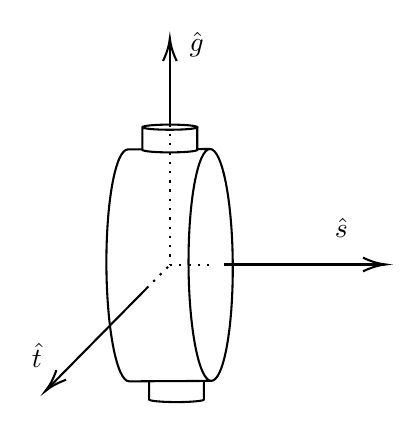
\begin{tikzpicture}[x=0.75pt,y=0.75pt,yscale=-1,xscale=1]
%uncomment if require: \path (0,249); %set diagram left start at 0, and has height of 249

%Shape: Can [id:dp06527002916107127] 
\draw  [fill={rgb, 255:red, 255; green, 255; blue, 255 }  ,fill opacity=1 ] (342.4,199.14) -- (342.4,210.05) .. controls (342.4,210.73) and (336.49,211.29) .. (329.2,211.29) .. controls (321.91,211.29) and (316,210.73) .. (316,210.05) -- (316,199.14) .. controls (316,198.46) and (321.91,197.9) .. (329.2,197.9) .. controls (336.49,197.9) and (342.4,198.46) .. (342.4,199.14) .. controls (342.4,199.82) and (336.49,200.38) .. (329.2,200.38) .. controls (321.91,200.38) and (316,199.82) .. (316,199.14) ;
%Shape: Can [id:dp8096689677898681] 
\draw  [color={rgb, 255:red, 0; green, 0; blue, 0 }  ,draw opacity=1 ][fill={rgb, 255:red, 255; green, 255; blue, 255 }  ,fill opacity=1 ] (345.97,201.08) -- (306.4,201.3) .. controls (300.52,201.33) and (295.61,176.35) .. (295.43,145.49) .. controls (295.26,114.64) and (299.89,89.6) .. (305.78,89.57) -- (345.34,89.35) .. controls (351.23,89.31) and (356.14,114.3) .. (356.31,145.15) .. controls (356.48,176.01) and (351.85,201.04) .. (345.97,201.08) .. controls (340.08,201.11) and (335.17,176.12) .. (335,145.27) .. controls (334.83,114.42) and (339.46,89.38) .. (345.34,89.35) ;
%Shape: Can [id:dp5210820858304941] 
\draw  [fill={rgb, 255:red, 255; green, 255; blue, 255 }  ,fill opacity=1 ] (339.2,78.84) -- (339.2,89.75) .. controls (339.2,90.43) and (333.29,90.99) .. (326,90.99) .. controls (318.71,90.99) and (312.8,90.43) .. (312.8,89.75) -- (312.8,78.84) .. controls (312.8,78.16) and (318.71,77.6) .. (326,77.6) .. controls (333.29,77.6) and (339.2,78.16) .. (339.2,78.84) .. controls (339.2,79.53) and (333.29,80.08) .. (326,80.08) .. controls (318.71,80.08) and (312.8,79.53) .. (312.8,78.84) ;
%Straight Lines [id:da7302123237400429] 
\draw  [dash pattern={on 0.84pt off 2.51pt}]  (314.87,156.42) -- (326,145.29) ;
%Straight Lines [id:da6678919295963763] 
\draw  [dash pattern={on 0.84pt off 2.51pt}]  (326,145.29) -- (348,145.29) ;
%Straight Lines [id:da12300205948280718] 
\draw  [dash pattern={on 0.84pt off 2.51pt}]  (326,77.6) -- (326,145.29) ;
%Straight Lines [id:da7145265678364978] 
\draw    (352,145) -- (428,145) ;
\draw [shift={(430,145)}, rotate = 180] [color={rgb, 255:red, 0; green, 0; blue, 0 }  ][line width=0.75]    (10.93,-3.29) .. controls (6.95,-1.4) and (3.31,-0.3) .. (0,0) .. controls (3.31,0.3) and (6.95,1.4) .. (10.93,3.29)   ;
%Straight Lines [id:da06879773433820491] 
\draw    (314.87,156.42) -- (267.4,204.58) ;
\draw [shift={(266,206)}, rotate = 314.59000000000003] [color={rgb, 255:red, 0; green, 0; blue, 0 }  ][line width=0.75]    (10.93,-3.29) .. controls (6.95,-1.4) and (3.31,-0.3) .. (0,0) .. controls (3.31,0.3) and (6.95,1.4) .. (10.93,3.29)   ;
%Straight Lines [id:da9989157109226341] 
\draw    (326,77.6) -- (326,38) ;
\draw [shift={(326,36)}, rotate = 450] [color={rgb, 255:red, 0; green, 0; blue, 0 }  ][line width=0.75]    (10.93,-3.29) .. controls (6.95,-1.4) and (3.31,-0.3) .. (0,0) .. controls (3.31,0.3) and (6.95,1.4) .. (10.93,3.29)   ;

% Text Node
\draw (404,121.4) node [anchor=north west][inner sep=0.75pt]    {$\hat{s}$};
% Text Node
\draw (334,31.4) node [anchor=north west][inner sep=0.75pt]    {$\hat{g}$};
% Text Node
\draw (258,181.4) node [anchor=north west][inner sep=0.75pt]    {$\hat{t}$};

\end{tikzpicture}
    \caption{Axis definition for Control Moment Gyroscope}
    \label{fig:tikCMG}
\end{figure}

\begin{figure}[!h]
    \centering
    

\tikzset{every picture/.style={line width=0.75pt}} %set default line width to 0.75pt        

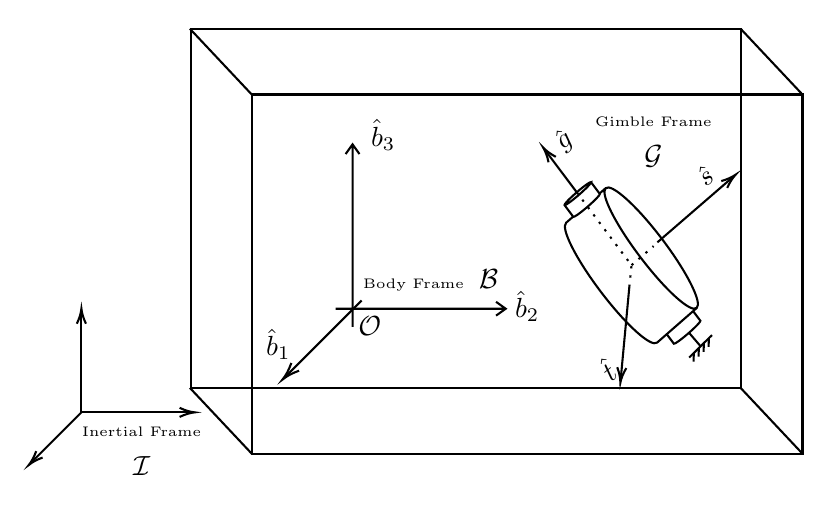
\begin{tikzpicture}[x=0.5pt,y=0.5pt,yscale=-1,xscale=1]
%uncomment if require: \path (0,350); %set diagram left start at 0, and has height of 350

%Shape: Can [id:dp8331189729524409] 
\draw  [fill={rgb, 255:red, 255; green, 255; blue, 255 }  ,fill opacity=1 ] (495.82,215.43) -- (502.2,223.92) .. controls (502.6,224.46) and (498.63,228.59) .. (493.34,233.17) .. controls (488.05,237.74) and (483.44,241.02) .. (483.04,240.49) -- (476.66,231.99) .. controls (476.26,231.46) and (480.23,227.32) .. (485.52,222.75) .. controls (490.81,218.17) and (495.42,214.9) .. (495.82,215.43) .. controls (496.22,215.96) and (492.25,220.1) .. (486.97,224.67) .. controls (481.68,229.25) and (477.06,232.52) .. (476.66,231.99) ;
%Shape: Can [id:dp8805062966141313] 
\draw  [color={rgb, 255:red, 0; green, 0; blue, 0 }  ,draw opacity=1 ][fill={rgb, 255:red, 255; green, 255; blue, 255 }  ,fill opacity=1 ] (499.54,214.7) -- (470.96,239.69) .. controls (466.71,243.41) and (448.54,227.03) .. (430.38,203.12) .. controls (412.22,179.2) and (400.94,156.79) .. (405.19,153.08) -- (433.77,128.08) .. controls (438.02,124.37) and (456.19,140.74) .. (474.35,164.66) .. controls (492.51,188.58) and (503.79,210.99) .. (499.54,214.7) .. controls (495.29,218.42) and (477.12,202.04) .. (458.96,178.12) .. controls (440.79,154.21) and (429.52,131.8) .. (433.77,128.08) ;
%Shape: Can [id:dp6975809963098918] 
\draw  [fill={rgb, 255:red, 255; green, 255; blue, 255 }  ,fill opacity=1 ] (423.17,123.76) -- (429.54,132.26) .. controls (429.94,132.79) and (425.98,136.93) .. (420.69,141.5) .. controls (415.4,146.07) and (410.79,149.35) .. (410.39,148.82) -- (404.01,140.32) .. controls (403.61,139.79) and (407.58,135.65) .. (412.86,131.08) .. controls (418.15,126.5) and (422.77,123.23) .. (423.17,123.76) .. controls (423.57,124.29) and (419.6,128.43) .. (414.31,133.01) .. controls (409.02,137.58) and (404.41,140.86) .. (404.01,140.32) ;
%Straight Lines [id:da7548151699735375] 
\draw  [dash pattern={on 0.84pt off 2.51pt}]  (450.87,199.43) -- (452.44,183.78) ;
%Straight Lines [id:da4676995296398143] 
\draw  [dash pattern={on 0.84pt off 2.51pt}]  (452.44,183.78) -- (468.4,169.98) ;
%Straight Lines [id:da24364084418605625] 
\draw  [dash pattern={on 0.84pt off 2.51pt}]  (412.86,131.08) -- (452.44,183.78) ;
%Straight Lines [id:da603601196492777] 
\draw    (471.13,167.25) -- (526.21,119.62) ;
\draw [shift={(527.73,118.31)}, rotate = 499.15] [color={rgb, 255:red, 0; green, 0; blue, 0 }  ][line width=0.75]    (10.93,-3.29) .. controls (6.95,-1.4) and (3.31,-0.3) .. (0,0) .. controls (3.31,0.3) and (6.95,1.4) .. (10.93,3.29)   ;
%Straight Lines [id:da39680954875025143] 
\draw    (450.87,199.43) -- (444.58,266.71) ;
\draw [shift={(444.39,268.7)}, rotate = 275.34000000000003] [color={rgb, 255:red, 0; green, 0; blue, 0 }  ][line width=0.75]    (10.93,-3.29) .. controls (6.95,-1.4) and (3.31,-0.3) .. (0,0) .. controls (3.31,0.3) and (6.95,1.4) .. (10.93,3.29)   ;
%Straight Lines [id:da931335338150046] 
\draw    (412.86,131.08) -- (389.74,100.28) ;
\draw [shift={(388.54,98.68)}, rotate = 413.1] [color={rgb, 255:red, 0; green, 0; blue, 0 }  ][line width=0.75]    (10.93,-3.29) .. controls (6.95,-1.4) and (3.31,-0.3) .. (0,0) .. controls (3.31,0.3) and (6.95,1.4) .. (10.93,3.29)   ;
%Straight Lines [id:da06748543672273133] 
\draw    (510.61,234.25) -- (494.14,250.49) ;
%Straight Lines [id:da33848315956607067] 
\draw    (493.86,232.43) -- (502.38,242.37) ;
%Straight Lines [id:da9582167503794932] 
\draw    (501.06,243.67) -- (500.93,249.9) ;
%Straight Lines [id:da1212417766847036] 
\draw    (497.44,247.24) -- (497.31,253.48) ;
%Straight Lines [id:da09420728047826432] 
\draw    (508.3,236.52) -- (508.18,242.76) ;
%Straight Lines [id:da8325536037855037] 
\draw    (504.68,240.09) -- (504.56,246.33) ;


%Shape: Rectangle [id:dp2711095269864183] 
\draw   (134,12.86) -- (531.27,12.86) -- (531.27,272.43) -- (134,272.43) -- cycle ;
%Shape: Rectangle [id:dp9597125724935636] 
\draw   (178,60.43) -- (576,60.43) -- (576,320) -- (178,320) -- cycle ;
%Straight Lines [id:da6047312216963134] 
\draw    (133.27,12.86) -- (178,60.43) ;
%Straight Lines [id:da614844554115443] 
\draw    (531.27,12.86) -- (576,60.43) ;
%Straight Lines [id:da9657702374196164] 
\draw    (133.27,272.43) -- (178,320) ;
%Straight Lines [id:da4943938352124151] 
\draw    (531.27,272.43) -- (576,320) ;
%Shape: Axis 2D [id:dp8483204934107569] 
\draw  (238.54,215.23) -- (361.54,215.23)(250.84,96.43) -- (250.84,228.43) (354.54,210.23) -- (361.54,215.23) -- (354.54,220.23) (245.84,103.43) -- (250.84,96.43) -- (255.84,103.43)  ;
%Straight Lines [id:da10965728905002736] 
\draw    (257.39,209.23) -- (201.53,265.09) ;
\draw [shift={(200.12,266.5)}, rotate = 315] [color={rgb, 255:red, 0; green, 0; blue, 0 }  ][line width=0.75]    (13.12,-3.95) .. controls (8.34,-1.68) and (3.97,-0.36) .. (0,0) .. controls (3.97,0.36) and (8.34,1.68) .. (13.12,3.95)   ;
%Straight Lines [id:da6362005944191291] 
\draw    (54.88,290.12) -- (18.21,326.79) ;
\draw [shift={(16.8,328.2)}, rotate = 315] [color={rgb, 255:red, 0; green, 0; blue, 0 }  ][line width=0.75]    (10.93,-3.29) .. controls (6.95,-1.4) and (3.31,-0.3) .. (0,0) .. controls (3.31,0.3) and (6.95,1.4) .. (10.93,3.29)   ;
%Straight Lines [id:da9762169812039505] 
\draw    (54.88,290.12) -- (134.8,290.12) ;
\draw [shift={(136.8,290.12)}, rotate = 180] [color={rgb, 255:red, 0; green, 0; blue, 0 }  ][line width=0.75]    (10.93,-3.29) .. controls (6.95,-1.4) and (3.31,-0.3) .. (0,0) .. controls (3.31,0.3) and (6.95,1.4) .. (10.93,3.29)   ;
%Straight Lines [id:da8439523067648185] 
\draw    (54.88,290.12) -- (54.88,217.11) ;
\draw [shift={(54.88,215.11)}, rotate = 450] [color={rgb, 255:red, 0; green, 0; blue, 0 }  ][line width=0.75]    (10.93,-3.29) .. controls (6.95,-1.4) and (3.31,-0.3) .. (0,0) .. controls (3.31,0.3) and (6.95,1.4) .. (10.93,3.29)   ;

% Text Node
\draw (459.47,94.83) node [anchor=north west][inner sep=0.75pt]    {$\mathcal{G} $};
% Text Node
\draw (423.88,74.43) node [anchor=north west][inner sep=0.75pt]   [align=left] {{\selectfont {\tiny Gimble Frame}}};
% Text Node
\draw (256.21,191.43) node [anchor=north west][inner sep=0.75pt]   [align=left] {{\selectfont {\tiny Body Frame}}};
% Text Node
\draw (186.18,227.83) node [anchor=north west][inner sep=0.75pt]    {$\hat{b}_{1}$};
% Text Node
\draw (366,200.4) node [anchor=north west][inner sep=0.75pt]    {$\hat{b}_{2}$};
% Text Node
\draw (262,76.4) node [anchor=north west][inner sep=0.75pt]    {$\hat{b}_{3}$};
% Text Node
\draw (340,185.0) node [anchor=north west][inner sep=0.75pt]    {$\mathcal{B} $};
% Text Node
\draw (494.35,116.24) node [anchor=north west][inner sep=0.75pt]  [rotate=-321.14]  {$\hat{s}$};
% Text Node
\draw (390.94,90.08) node [anchor=north west][inner sep=0.75pt]  [rotate=-321.14]  {$\hat{g}$};
% Text Node
\draw (423.5,254.57) node [anchor=north west][inner sep=0.75pt]  [rotate=-321.14]  {$\hat{t}$};
% Text Node
\draw (252.84,218.63) node [anchor=north west][inner sep=0.75pt]    {$\mathcal{O} $};
% Text Node
\draw (53.21,298.43) node [anchor=north west][inner sep=0.75pt]   [align=left] {{\selectfont {\tiny Inertial Frame}}};
% Text Node
\draw (90,320) node [anchor=north west][inner sep=0.75pt]    {$\mathcal{I} $};

\end{tikzpicture}

    \caption{Axis definition for Spacecraft Body with \acrfull{vscmg}}
    \label{fig:tikCMG}
\end{figure}
\usetikzlibrary{shapes}
\tdplotsetmaincoords{60}{120}


\begin{equation*}
A\hat{s} =
\begin{bmatrix}
\cos(\beta) \cos(\delta_1) & -\sin(\delta_2) & -\cos(\beta) \cos(\delta_3) &  \sin(\delta_4) \\
-\sin(\delta_1) & -\cos(\beta) \cos(\delta_2) &  \sin(\delta_3) &  \cos(\beta) \cos(\delta_4) \\
\sin(\beta) \cos(\delta_1) &  \sin(\beta) \cos(\delta_2) &  \sin(\beta) \cos(\delta_3) &  \sin(\beta) \cos(\delta_4) 
\end{bmatrix}
\end{equation*}
\begin{equation*}
A\hat{t} =
\begin{bmatrix}
\cos(\beta) \sin(\delta_1) &         \cos(\delta_2) & -\cos(\beta) \sin(\delta_3) &       -\cos(\delta_4) \\
       \cos(\delta_1) & -\cos(\beta) \sin(\delta_2) &        -\cos(\delta_3) & \cos(\beta) \sin(\delta_4) \\
\sin(\beta) \sin(\delta_1) &  \sin(\beta) \sin(\delta_2) &  \sin(\beta) \sin(\delta_3) & \sin(\beta) \sin(\delta_4)

\end{bmatrix}
\end{equation*}
\begin{equation*}
A\hat{g} = 
\begin{bmatrix}
 -\sin(\beta) &      0 & \sin(\beta) &       0 \\
       0 & \sin(\beta) &      0 & -\sin(\beta) \\
  \cos(\beta) & \cos(\beta) & \cos(\beta) &  \cos(\beta)
\end{bmatrix}
\end{equation*}



\tikzset{every picture/.style={line width=0.75pt}} %set default line width to 0.75pt        
\begin{figure}[ht]
\centering
\newcommand{\AxisRotator}[1][rotate=0]{%
    \tikz [x=0.25cm,y=0.60cm,line width=.1ex,-stealth,#1] \draw (0,0) arc (-150:150:1 and 1);%
}

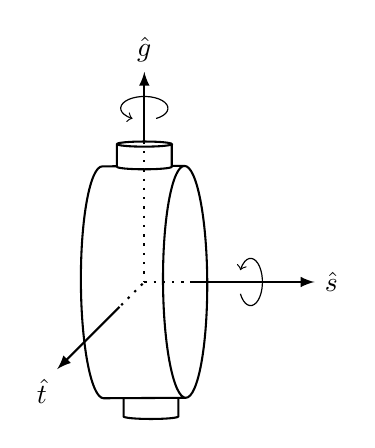
\begin{tikzpicture}[x=0.75pt,y=0.75pt,yscale=-1,xscale=1]
%uncomment if require: \path (0,284); %set diagram left start at 0, and has height of 284

%Shape: Can [id:dp7170334139971102] 
\draw  [fill={rgb, 255:red, 255; green, 255; blue, 255 }  ,fill opacity=1 ] (260.4,169.85) -- (260.4,180.76) .. controls (260.4,181.45) and (254.49,182) .. (247.2,182) .. controls (239.91,182) and (234,181.45) .. (234,180.76) -- (234,169.85) .. controls (234,169.17) and (239.91,168.62) .. (247.2,168.62) .. controls (254.49,168.62) and (260.4,169.17) .. (260.4,169.85) .. controls (260.4,170.54) and (254.49,171.09) .. (247.2,171.09) .. controls (239.91,171.09) and (234,170.54) .. (234,169.85) ;
%Shape: Can [id:dp8604613691481404] 
\draw  [color={rgb, 255:red, 0; green, 0; blue, 0 }  ,draw opacity=1 ][fill={rgb, 255:red, 255; green, 255; blue, 255 }  ,fill opacity=1 ] (263.97,171.79) -- (224.4,172.01) .. controls (218.52,172.04) and (213.61,147.06) .. (213.43,116.2) .. controls (213.26,85.35) and (217.89,60.31) .. (223.78,60.28) -- (263.34,60.06) .. controls (269.23,60.03) and (274.14,85.01) .. (274.31,115.86) .. controls (274.48,146.72) and (269.85,171.76) .. (263.97,171.79) .. controls (258.08,171.82) and (253.17,146.84) .. (253,115.98) .. controls (252.83,85.13) and (257.46,60.09) .. (263.34,60.06) ;
%Shape: Can [id:dp28656579674299] 
\draw  [fill={rgb, 255:red, 255; green, 255; blue, 255 }  ,fill opacity=1 ] (257.2,49.55) -- (257.2,60.46) .. controls (257.2,61.15) and (251.29,61.7) .. (244,61.7) .. controls (236.71,61.7) and (230.8,61.15) .. (230.8,60.46) -- (230.8,49.55) .. controls (230.8,48.87) and (236.71,48.32) .. (244,48.32) .. controls (251.29,48.32) and (257.2,48.87) .. (257.2,49.55) .. controls (257.2,50.24) and (251.29,50.79) .. (244,50.79) .. controls (236.71,50.79) and (230.8,50.24) .. (230.8,49.55) ;
%Straight Lines [id:da6813117542504483] 
\draw  [dash pattern={on 0.84pt off 2.51pt}]  (232.87,127.13) -- (244,116) ;
%Straight Lines [id:da7942658869494881] 
\draw  [dash pattern={on 0.84pt off 2.51pt}]  (244,116) -- (266,116);
%Straight Lines [id:da8094718055923082] 
\draw  [dash pattern={on 0.84pt off 2.51pt}]  (244,48.32) -- (244,116) ;

%Straight Lines [id:da10899843254419173] 
\draw[-latex]    (266,116) -- (326,116) node[anchor=west] {$\hat{s}$} node [midway] {\AxisRotator[x=0.15cm,y=0.3cm,->,rotate=0,black]} ;
%Straight Lines [id:da31922966493534966] 
\draw[-latex]    (232,128) -- (202,158) node[anchor=north east] {$\hat{t}$};
%Straight Lines [id:da6086340922936091] 
\draw[-latex]    (244,48.32) -- (244,14.71) node[above] {$\hat{g}$} node [midway] {\AxisRotator[x=0.15cm,y=0.3cm,->,rotate=90,black]};


\end{tikzpicture}
\caption{Single Gimble Control Moment Gyroscope basis vectors, initialy each SGCMG's wheel spin axis is facing towards x of pyramid, gimble axis is aligned with z axis}
\label{fig:sgcmg}
\end{figure}

\subsection{Satellite Attitude Dynamics}
\subsection{RW}
\subsection{CMG}
\subsection{VSCMG}
